% Generated by Listas/make_statements.py from pratica-lecture-08.md, item 11. Do not edit.
\textbf{Source.} Muñoz-Garcia \& Toro-Gonzalez (2019), \emph{Strategy and Game Theory: Practice Exercises with Answers}, Ch. 9, Exercise 5 ``Finding Semi-Separating Equilibrium'', pp.~422--423 {[}PDF pp.~431--432{]}. Reproduced verbatim (statement only; the book's worked answer follows it). ``Obviously, player makes his choice'' is as printed. Answer: yes, the book's worked answer follows the exercise.



\begin{quote}

Consider the sequential game with incomplete information depicted in Fig. 9.46. Two players are playing the following super-simple poker game. The first player gets his cards, and obviously he is the only one who can observe them. He can either get a High hand or a Low hand, with equal probabilities. After observing his hand, he must decide whether to Bet (let us imagine that he is betting a fixed amount of a dollar) or Resign from the game. If he resigns his payoff is \(-1\), independent of whether he has a High or a Low hand, and player 2 gets a dollar. If he bets, player 2 must decide whether to Call or Fold from the game. Obviously, player makes his choice without being able to observe player 1's hands, but only observing that player 1 Bets.



\pandocbounded{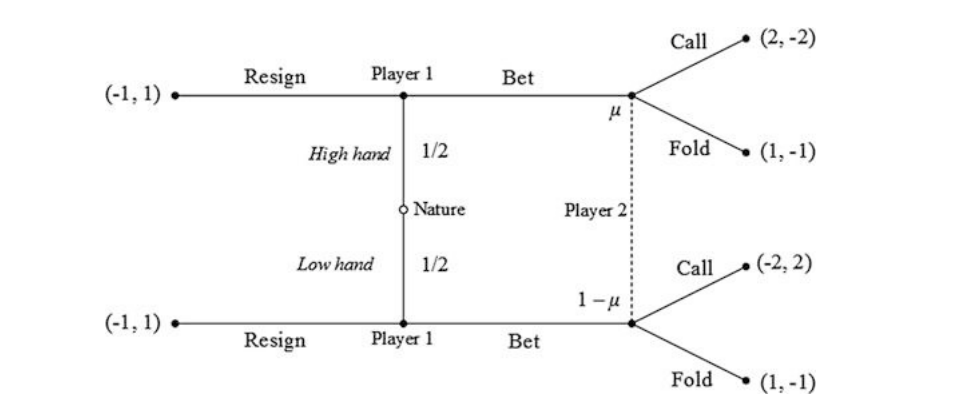
\includegraphics[keepaspectratio,alt={Fig. 9.46 A simple poker game}]{../figures/munoz-garcia-9-5.png}}



\emph{Fig. 9.46} A simple poker game



\begin{enumerate}

\def\labelenumi{(\alph{enumi})}

\item

  Show that no separating PBE can be sustained where player 1 chooses a pure strategy (i.e., betting or resigning, given his cards, with 100\% probability).

\item

  Show that no pooling PBE can be sustained where player 1 chooses a pure strategy (i.e., betting or resigning, given his cards, with 100\% probability).

\item

  Find a semi-separating PBE where player 1 chooses Bet or Resign in pure strategies when having a high hand, but randomizes between bet and resign when having a low hand.

\end{enumerate}

\end{quote}

